\section{Problem 1: Secure PRP}\label{sec:problem1}

Suppose $F$ is a secure PRP with blocklength $\lambda$.
Give the decryption algorithm for the following scheme and prove that it does not have CPA security:

\begin{figure}[h!]
    \centering
\begin{minipage}[t]{.45\textwidth}
\null 
 \begin{algorithm}[H]
    \DontPrintSemicolon
    $\mathcal{K} \gets \{\textcolor{red}{0}, \textcolor{red}{1}\}^{\lambda}$ \;
    $\mathcal{M} \gets \{ \textcolor{red}{0} , \textcolor{red}{1} \}^{2\lambda}$ \;
    $\mathcal{C} \gets \left( \{ \textcolor{red}{0} , \textcolor{red}{1} \}^{\lambda}\right)^3$ \;
    \Begin{
        $k \gets \{ \textcolor{red}{0}, \textcolor{red}{1} \}^{\lambda} $ \;
        \KwRet{$k$}
    }
    \caption{Key generation procedure}
  \end{algorithm}
\end{minipage}%
\begin{minipage}[t]{.45\textwidth}
\null
 \begin{algorithm}[H]
    \DontPrintSemicolon
    \Begin{
        $r \gets \{ \textcolor{purple}{0} , \textcolor{purple}{1} \}^\lambda$ \;
        $s \gets F_k (r \oplus m_1)$ \;
        $t \gets F_k (r \oplus m_1 \oplus F_k (m_1) \oplus m_2)$ \;
        $c \gets \langle r$ $\vert \vert$ $s$ $\vert \vert$ $t \rangle$ \;
        \KwRet{$c$}
    }
     \vspace{4.4pt}
    \caption{Encryption algorithm}
  \end{algorithm}
\end{minipage}
    \caption{Encryption and key generation scheme for Problem 1.\label{prob1:encryption}}
\end{figure}
\begin{center}
    \rule{5cm}{0.4pt}
\end{center}

\textbf{\textit{Proof:}}
For the decryption algorithm, we will assume we are given the pseudo-random permutation F and its associated key $k$.
We also assume access to the cipher text, which consists of a concatenation of 3 parameters: $r$, $s$ and $t$.
Lastly, the plain text will be of the form $m = \langle m_1$ $\vert \vert$ $m_2 \rangle$.

To find each of its two parts we will isolate them from the $s$ and $t$ expressions.
This can be easily done as F is a secure PRP and, therefore, efficiently invertible.
Also, the $\oplus$ (XOR) operator can be inverted using the relation $a \oplus b = c \Leftrightarrow a = c \oplus b$.
The full decryption algorithm for the encryption scheme in Figure~\ref{prob1:encryption} is depicted in Algorithm~\ref{fig1:decryption}.
\begin{algorithm}
    \DontPrintSemicolon
    \KwData{Cipher text composed of three parameters - $r$, $s$, and $t$ - concatenated together.}
    \KwResult{Plain text $m$}
    \Begin{
        $m_1 \gets F_k^{-1} (s) \oplus r; \hspace{5pt}$\;
        $m_2 \gets F_k^{-1} (t) \oplus r \oplus m_1 \oplus F_k (m_1)$ \;
        $m \gets \langle m_1 \vert \vert m_2 \rangle $ \;
        \KwRet{$m$}
    }
    \caption{Decryption algorithm for the given scheme.\label{fig1:decryption}}
\end{algorithm}

To verify the correctness of the decryption algorithm, we can check that $Dec_k (Enc_k (m)) = m$, for every message $m \in \mathcal{M}$.

%Now, to show that this scheme is not CPA-secure, we need to put ourselves in the adversary's shoes. This means that we no longer have access to the PRP, nor the private key $k$, but we are able to know the ciphertext associated to a chosen plaintext, for various queries.

%One of the main techniques that witnesses a non CPA-secure scheme is to check that it is deterministic (not randomized). Clearly, this one is not the case, so we'll have to think it twice.
To prove that the scheme from Figure~\ref{prob1:encryption} is not CPA secure we will use the attack game depicted in Figure~\ref{prob1:attack-game}.

\begin{figure}[h!]
    \centering
    \begin{tikzpicture}
        % Define Variables
        \def\lR{0.75}
        \def\rR{9.35}
        \def\bottom{-9.5}

        % Overall Scheme
        \draw[thick] (0,0) -- (10,0) node[midway, anchor=south] {PRF Game $4.2$};
        \node[anchor = north west] at (0,0) (c-r) {Challenger};
        \draw[dotted] (\lR, -0.5) -- (\lR,\bottom);
        \node[anchor = north east] at (10,0) {Attacker};
        \draw[dotted] (\rR, -0.5) -- (\rR, \bottom);

        % 1st Query
        \draw[->] (\rR, -1) -- (\lR, -1) node[midway, anchor=south] {\textbf{1st Query}} node[midway, anchor=north, align=center] {$M_{10} \gets \langle m_1 \vert \vert m_2 \rangle$ \\ $M_{11} \gets \langle m_1 \vert \vert \hat{m_2} \rangle$};
        \node[anchor=west, align=left] at (\lR, -2.5) {$b \overset{\mathcal{R}}{\longleftarrow} \{0,1\}$ \\ $c_1 \gets \text{Enc}_k \left( M_{1b} \right) = \langle r \vert \vert s \vert \vert t \rangle$};
        \draw[->] (\lR, -3.5) -- (\rR, -3.5) node[midway, anchor=south] {\textbf{$c_1$}};

        % 2nd Query
        \draw[->] (\rR, -5) -- (\lR, -5) node[midway, anchor=south] {\textbf{2nd Query}} node[midway, anchor=north, align=center] {$M_{20} \gets \langle r_1 \oplus m_1 \vert \vert s \rangle$ \\ $M_{21} \gets \langle r_1 \oplus m_1 \vert \vert p \rangle$};
        \node[anchor=west, align=left] at (\lR, -6.5) {$b' \overset{\mathcal{R}}{\longleftarrow} \{0,1\}$ \\ $c_2 \gets \text{Enc}_k \left( M_{2b'} \right) = \langle r' \vert \vert s' \vert \vert t' \rangle$};
        \draw[->] (\lR, -7.5) -- (\rR, -7.5) node[midway, anchor=south] {\textbf{$c_2$}};

        % Forgery
        \node[anchor=east, align=right] at (\rR, -8.5) {$\hat{b} \gets \left\lbrace \begin{array}{l} 0 \text{ if } s' = t' \\ 1 \text{ if } s' \neq t' \end{array} \right\rbrace$};
        \draw[->] (\rR, -9.25) -- (\lR, -9.25) node[midway, anchor=south] {$\hat{b}$};

    \end{tikzpicture}
    \caption{Attack to the $CPA$ game.\label{prob1:attack-game}}
\end{figure}

Let's recall that a cipher $\mathcal{E}$ is \textbf{CPA-secure} (or semantically secure against chosen plaintext attack) if, for all efficient adversaries $\mathcal{A}$, the value CPAadv$[\mathcal{A}, \mathcal{E}]$ is negligible.
We will work instead with the "bit guessing" game version described in Boneh \& Shoup's book. In this similar version, we have the following advantage, for a $b \in \{0, 1\}$ randomly selected by the challenger and the $\hat b \in \{0, 1\}$ computed by the adversary:

\begin{equation*}
    \text{CPAadv}[\mathcal{A}, \mathcal{E}] = 2 \cdot \text{CPAadv}^{*}[\mathcal{A}, \mathcal{E}] = 2 \cdot \left| \mathbb{P}[\hat{b} = b] - \frac{1}{2} \right|
\end{equation*}

Now, we build an smart adversary that only takes 2 queries to break the CPA security: in the first attempt, they will send the messages $M = <m_1$ $\vert \vert$ $m_2>$ and $\hat M = <m_1$ $\vert \vert$ $\hat m_2>$, meaning that in both cases the challenger will return the same $s := F_k (r \oplus m_1)$, altogether with the first generated random number $r$.

Now the adversary has access to a valuous information: $r \oplus m_1$ (since they have both strings) and its pseudo-random permutation $s = F_k (r \oplus m_1)$.
The second query will consist of the two messages $M' = <r \oplus m_1$ $\vert \vert$ $s>$ and $\hat M' = <r \oplus m_1$ $\vert \vert$ $p>$, where $p$ is any string other than $s$.
From the challenger, the adversary will receive the new values $r'$ (again, randomly generated), $s' := F_k(r' \oplus r \oplus m_1)$ and $t' := F_k(r' \oplus (r \oplus m_1) \oplus F_k (r \oplus m_1) \oplus m_x)$, where $m_x$ could either be $s$ or $p$ with equal probability.

The key idea now is to see that the messages $s'$ and $t'$ will be exactly the same if and only if the message selected by the challenger is $m_x = s$.
This happens because $F_k(r \oplus m_1) \oplus s = 1$, which leads to $t' = F_k(r' \oplus r \oplus m_1) = s'$.
And this happens exclusively for $m_x = s$ since F is a permutation and, therefore, gives different outputs for different inputs.

That means in the second query the adversary is capable to find the correct $\hat b$ with probability $1$, leading to $\text{CPAadv}[\mathcal{A}, \mathcal{E}] = 2 \cdot \vert \mathbb{P}[\hat{b} = b] - \frac{1}{2} \vert = 2 \cdot \vert 1 - \frac{1}{2} \vert = 1$, which is clearly not negligible, and the scheme is not CPA-secure. \hfill \qed

